\chapter{System Architecture}
\label{ch:system-architecture}

\section{Overall Architecture Overview}
The Mountain Climber Health and GPS Tracker system is built upon a multi-tiered architecture that seamlessly integrates edge computing devices, local communication meshes, and centralized visualization platforms. The architecture is designed to be highly resilient, ensuring continuous operation even in completely off-grid environments. It is broadly categorized into three distinct layers: the Hardware Layer, the Communication Layer, and the Application Layer.

\subsection{Layered Architecture}
\begin{itemize}
    \item \textbf{Hardware Layer:} This is the physical foundation of the system, comprising the edge devices worn by the climbers (Wristband and Main Device), the intermediate infrastructure (Repeaters), and the receiving end (Base Camp Unit). These devices are responsible for data acquisition (GPS, health vitals) and initial data processing.
    \item \textbf{Communication Layer:} Acting as the nervous system, this layer handles all data transmission between the hardware nodes. It utilizes a combination of Bluetooth Low Energy (BLE) for short-range personal area networks, a LoRa mesh network for long-range inter-node communication, and USB Serial for direct data transfer to the dashboard.
    \item \textbf{Application Layer:} This layer consists of the software interfaces used by the end-users. It includes the Flutter-based mobile application used by the climbers and the Python Flask desktop dashboard used by the base camp operators to monitor the expedition.
\end{itemize}

\section{System Block Diagram}
The following diagram illustrates the high-level interconnection between all system components.

\begin{figure}[htbp]
    \centering
    \begin{tikzpicture}[
        node distance=1cm and 1cm,
        box/.style={draw, rectangle, rounded corners, minimum width=2.2cm, minimum height=1.2cm, align=center, fill=blue!10, font=\scriptsize},
        arrow/.style={thick, ->, >=stealth}
    ]
        % Nodes
        \node[box] (wristband) {Wristband\\(ESP32, MAX30102)};
        \node[box, right=of wristband] (phone) {Smartphone App\\(Flutter/BLE)};
        \node[box, below=of wristband] (climber) {Climber Device\\(ESP32, GPS, LoRa)};
        \node[box, right=of climber] (repeater) {Repeater Node\\(ESP32, LoRa)};
        \node[box, right=of repeater] (basecamp) {Base Camp Unit\\(ESP32, LoRa)};
        \node[box, above=of basecamp] (dashboard) {Base Camp\\Dashboard\\(Flask/Python)};
        \node[box, above=of dashboard] (portal) {Web Portal\\(Next.js/Supabase)};

        % Connections
        \draw[arrow, <->, dashed] (wristband) -- node[above, font=\tiny] {BLE} (phone);
        \draw[arrow, <->] (phone) -- node[right, font=\tiny] {BLE} (climber);
        \draw[arrow, <->, thick, red] (climber) -- node[above, font=\tiny] {LoRa} (repeater);
        \draw[arrow, <->, thick, red] (repeater) -- node[above, font=\tiny] {LoRa} (basecamp);
        \draw[arrow, <->, thick] (basecamp) -- node[right, font=\tiny] {USB Serial} (dashboard);
        \draw[arrow, <->, dashed] (dashboard) -- node[right, font=\tiny] {WiFi/Internet} (portal);
        
    \end{tikzpicture}
    \caption{High-Level System Architecture and Interconnections}
    \label{fig:system-architecture}
\end{figure}

\begin{infobox}
The system operates completely independently of cellular networks during an expedition. Internet connectivity is only required for the Web Portal, which is used pre- and post-expedition for device registration and data sync.
\end{infobox}

\section{Data Flow Architecture}
Data flows through the system in two primary pipelines: health telemetry and geographical tracking/messaging.

\begin{figure}[htbp]
    \centering
    \begin{tikzpicture}[
        auto,
        block/.style={rectangle, draw=black, thick, fill=green!10, text width=5.5em, text centered, rounded corners, minimum height=3em, font=\scriptsize},
        line/.style={draw, thick, -latex, shorten >=2pt}
    ]
        % Define nodes
        \node [block] (sensor) {MAX30102 Sensor};
        \node [block, right=1cm of sensor] (wristband) {Wristband ESP32};
        \node [block, right=1cm of wristband] (phone) {Climber's Phone};
        \node [block, below=1cm of phone] (climber) {Main Climber Device};
        \node [block, left=1cm of climber] (gps) {NEO-6M GPS};
        \node [block, below=1cm of climber] (lora_mesh) {LoRa Mesh / Repeaters};
        \node [block, right=1.5cm of lora_mesh] (base_esp) {Base Camp ESP32};
        \node [block, above=1cm of base_esp] (dashboard) {Flask Dashboard};

        % Draw edges
        \path [line] (sensor) -- node[above, font=\tiny] {I2C} (wristband);
        \path [line] (wristband) -- node[above, font=\tiny] {BLE Adv.} (phone);
        \path [line] (phone) -- node[right, font=\tiny] {BLE} (climber);
        \path [line] (gps) -- node[above, font=\tiny] {UART} (climber);
        \path [line] (climber) -- node[right, font=\tiny] {LoRa TX} (lora_mesh);
        \path [line] (lora_mesh) -- node[above, font=\tiny] {LoRa RX} (base_esp);
        \path [line] (base_esp) -- node[right, font=\tiny] {Serial JSON} (dashboard);
        
    \end{tikzpicture}
    \caption{Detailed Data Flow Diagram}
    \label{fig:data-flow}
\end{figure}

The data flow begins at the edges:
\begin{enumerate}
    \item \textbf{Health Data:} The MAX30102 sensor on the Wristband reads raw photoplethysmogram (PPG) data, which the ESP32 processes to calculate Heart Rate and SpO$_2$. This data is advertised via BLE.
    \item \textbf{Local Aggregation:} The climber's mobile phone app scans for these BLE advertisements, displaying the vitals locally.
    \item \textbf{Transmission Prep:} The Main Climber Device, which is paired via BLE to the phone and directly reading GPS data via UART, constructs data packets containing the GPS coordinates, health vitals (received via the phone or direct BLE), and system status.
    \item \textbf{Long-Range Transmission:} These packets are broadcast over the 433 MHz LoRa interface.
    \item \textbf{Relay:} Repeater nodes pick up the LoRa packets and re-broadcast them, extending the range over rough terrain.
    \item \textbf{Reception \& Display:} The Base Camp Unit receives the LoRa packets, formats them into a serialized JSON structure, and pushes them over a USB serial connection (at 115200 baud) to the laptop running the Python Flask dashboard, which renders the data on an HTML5 canvas map.
\end{enumerate}

\section{Deployment Strategy in Mountainous Terrain}
The physical deployment of the hardware is critical to the system's success. LoRa, operating at 433 MHz, requires line-of-sight (LoS) or near-LoS for maximum range. In a mountain setting, valleys and ridges obstruct radio waves. 

\begin{figure}[htbp]
    \centering
    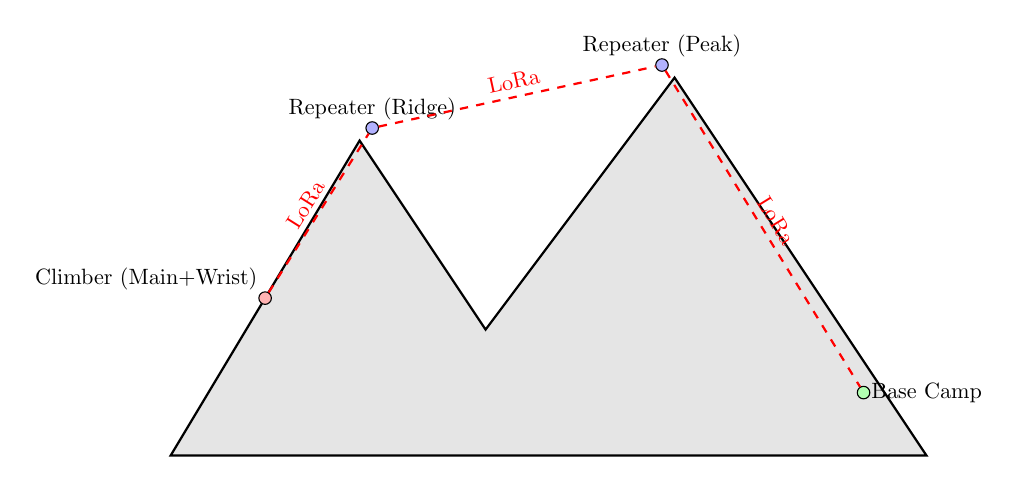
\begin{tikzpicture}[scale=0.8, transform shape]
        % Mountain drawing
        \draw[thick, fill=gray!20] (0,0) -- (3,5) -- (5,2) -- (8,6) -- (12,0) -- cycle;
        
        % Nodes
        \node[circle, draw, fill=red!30, inner sep=2pt] (climber) at (1.5,2.5) {};
        \node[above left] at (climber) {Climber (Main+Wrist)};
        
        \node[circle, draw, fill=blue!30, inner sep=2pt] (repeater1) at (3.2,5.2) {};
        \node[above] at (repeater1) {Repeater (Ridge)};
        
        \node[circle, draw, fill=blue!30, inner sep=2pt] (repeater2) at (7.8,6.2) {};
        \node[above] at (repeater2) {Repeater (Peak)};
        
        \node[circle, draw, fill=green!30, inner sep=2pt] (base) at (11,1) {};
        \node[right] at (base) {Base Camp};
        
        % LoRa links
        \draw[dashed, thick, red] (climber) -- node[above, sloped] {LoRa} (repeater1);
        \draw[dashed, thick, red] (repeater1) -- node[above, sloped] {LoRa} (repeater2);
        \draw[dashed, thick, red] (repeater2) -- node[above, sloped] {LoRa} (base);
        
    \end{tikzpicture}
    \caption{Deployment diagram illustrating the role of Repeaters in overcoming mountain topology}
    \label{fig:deployment}
\end{figure}

To overcome this, \textbf{Repeater Nodes} are strategically placed at high elevation points (e.g., ridges or peaks) during the ascent. These nodes act as relay stations. The base camp is typically located in a valley, and the climber may be on the other side of a ridge. The repeater on the ridge ensures continuous communication by acting as a bridge between the climber and the base camp.
